% Hermite's Problem: Complementary Solutions - Using generated figure

\begin{figure}[p]
\centering
\vspace{2cm}
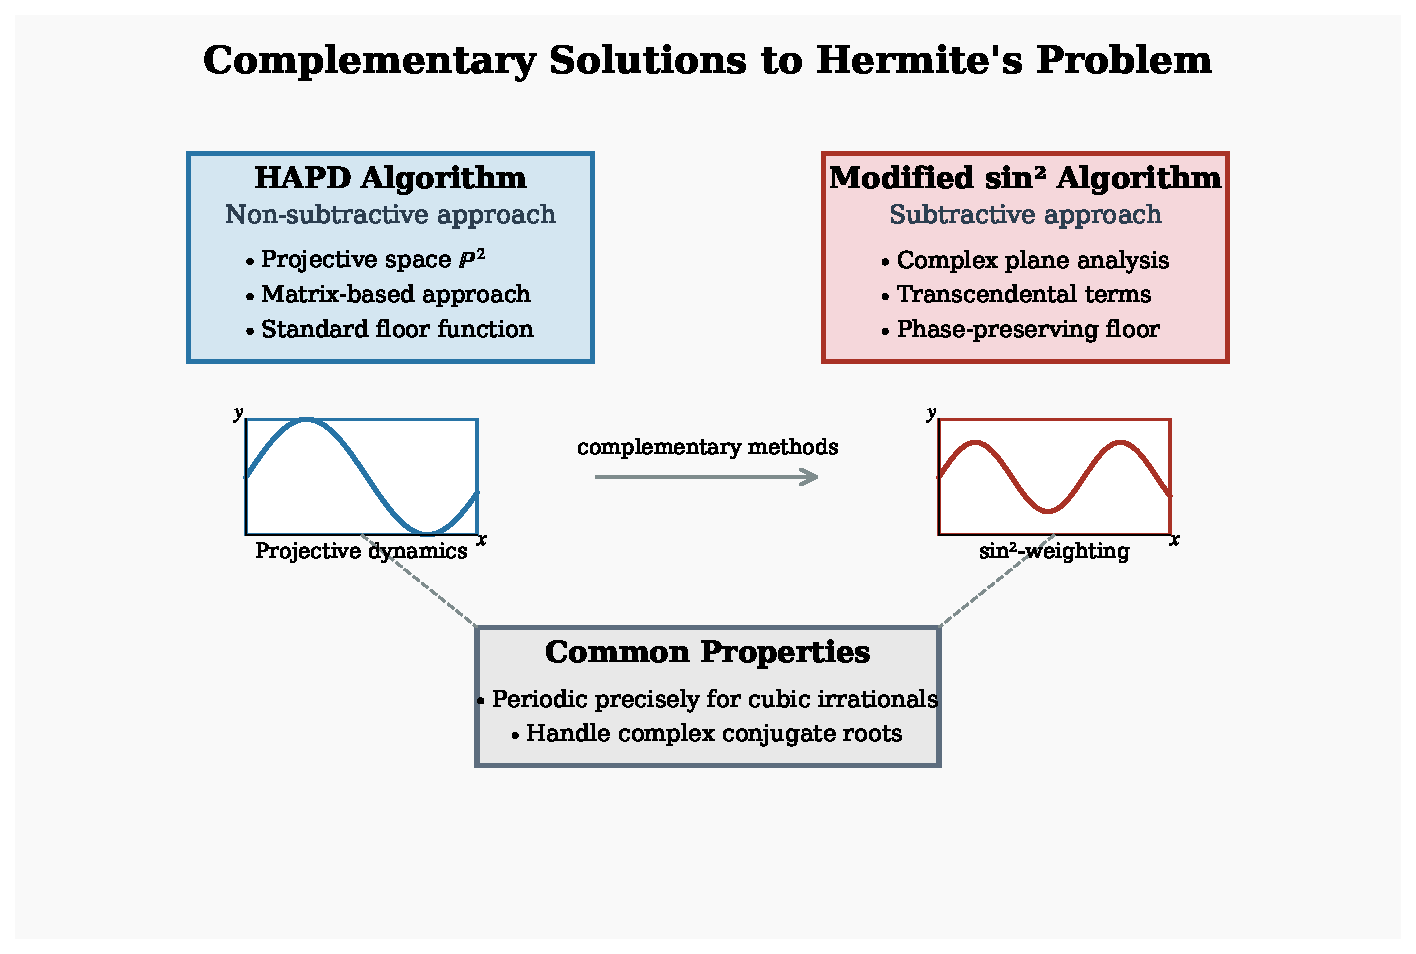
\includegraphics[width=0.85\textwidth]{figures/complementary_solutions_diagram.pdf}
\vspace{1.5cm}
\caption{Comparison of complementary approaches to Hermite's problem. The HAPD algorithm uses a non-subtractive approach in projective space with matrix-based techniques, while the Modified sin$^2$ algorithm employs a subtractive approach with transcendental functions in the complex plane. Both methods are effective at detecting periodicity in cubic irrationals despite their fundamentally different mathematical foundations.}
\label{fig:complementary_approaches}
\end{figure}
\clearpage

% Note: The image files (examples/graph_proj.pdf and examples/graph_sin.pdf) will need to be created or replaced with actual graphs.
% For compilation testing, comment out the \includegraphics lines or create simple placeholder graphics. 